\section{Stage 4: Extension Build} \label{sec:work_stage4_extension_build}

The last stage was to build an extension for an IDE, VSCode. This extension allows the user to have a better understanding of how much energy the code is consuming, and what are the methods, and variables that most affect it.
When opening the extension side page, it contains some sliders that can change the input values, and it has the estimate button, to predict the energy.
The sliders are updated when the document is saved.%, rather than on every change, to prevent performance slowdowns.

The extension analyzes the user's Java files, identifies all the methods used, and matches them against a set of pre-trained models. Then it finds which variables affect those methods, meaning the variables that are the inputs to the method, for example, in \texttt{list.add(i)}  the inputs and important variables are \texttt{list} and \texttt{i}.
The extension does this to every method it finds and groups it by method. In the end it creates groups of input variables for each method, and displays it in sliders. The sliders allow the user to change the input values and when pressing the estimate button, depending on the changed values, it will change the energy estimation.

If a method calls another user-defined method that already has an assigned energy cost (but is not a trained method), then the calling method will also include that energy cost.

When a trained method is called inside a loop, a new slider appears to represent the loop size. The method’s energy cost is multiplied by this loop size. In the case of nested loops, the energy cost is multiplied by the product of all nested loop sizes.

Note that only methods and variables that affect the energy appear on the panel.

\begin{figure}[htbp]
  \centering
  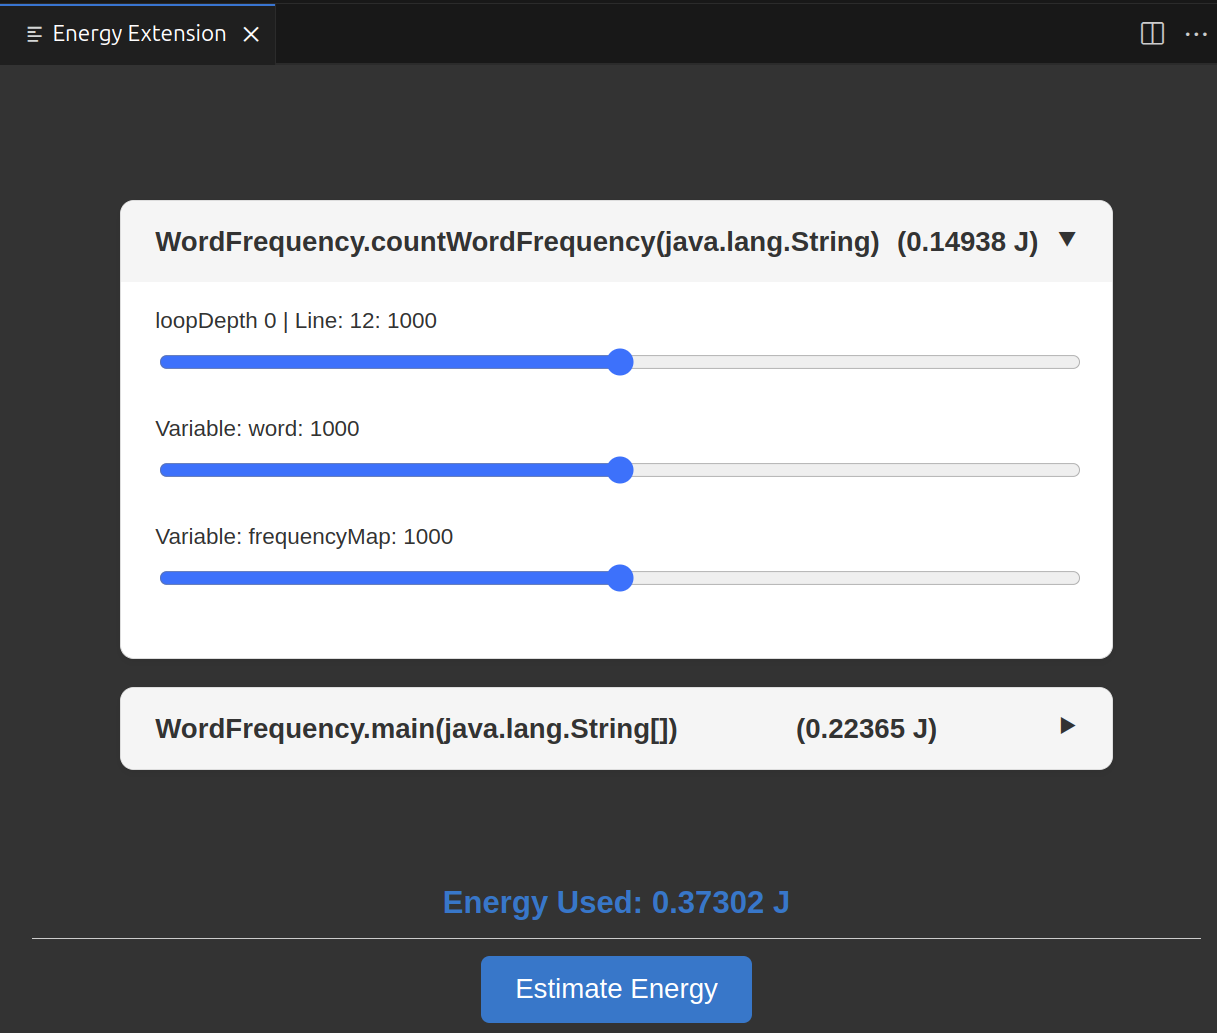
\includegraphics[width = .8 \textwidth]{figures/extension_example1.png}
  \caption{Extension example HashMap}
  \label{fig:extension_example1}
\end{figure}

This extension can help understand how much energy the code is using.
For example, this small code snippet ~\ref{lst:Java_program_to_count_word_frequencies_in_a_string} that counts how many times each word appears in a given text string, can be estimated for how much energy it uses.

\begin{listing}[H]
\begin{minted}[linenos, fontsize=\small, frame=none, bgcolor=white,breaklines=true,breakanywhere=true]{Java}
    public class WordFrequency {
    public static HashMap<String, Integer> countWordFrequency(String text) {
        String[] words = text.toLowerCase().split("\\W+");
        HashMap<String, Integer> frequencyMap = new HashMap<>();
        for (String word : words) {
            if (word.isEmpty()) continue; 
            frequencyMap.put(word, frequencyMap.getOrDefault(word, 0) + 1);
        }
        return frequencyMap;
    }
    public static void main(String[] args) {
        String input = "Java is simple. Java is powerful.";
        HashMap<String, Integer> result = countWordFrequency(input);
        System.out.println(result);
    }
}
\end{minted}
\caption{Java program to count word frequencies in a string}            
\label{lst:Java_program_to_count_word_frequencies_in_a_string}
\end{listing}

Using the energy prediction extension it is possible to understand how much energy this code uses, as it can be seen in the figure \ref{fig:extension_example1}.
In the figure 2 methods can be seen, and their energy is displayed, also one of the containers has the important variables that might affect the energy of the code. For instance, in the method \texttt{countWordFrequency(String)} it can be seen that the size of the variables \texttt{word} and \texttt{frequencyMap} can change the energy usage. Also, the loop size is taken into account, and the number operations performed will impact the energy significantly.
The 2 variables shown in the figure\ref{fig:extension_example1}, show up because of the method \texttt{Map.put(Object,Object)}, which means it will have 3 inputs. The first one is the collection input, (i.e \texttt{frequencyMap}), the second one is the first Object which is the variable \texttt{word} and the last Object is not a variable, so it does not appear in the extension.


If, for instance, instead of using \texttt{HashMap}, \texttt{TreeMap} is used, the energy differences can easily be noticed ~\ref{fig:extension_example2}. This shows a great example of how two implementations of the same collection can differ in energy. It can also be used to compare different method implementations, that achieve the same output but rely on different approaches.



\begin{figure}[htbp]
  \centering
  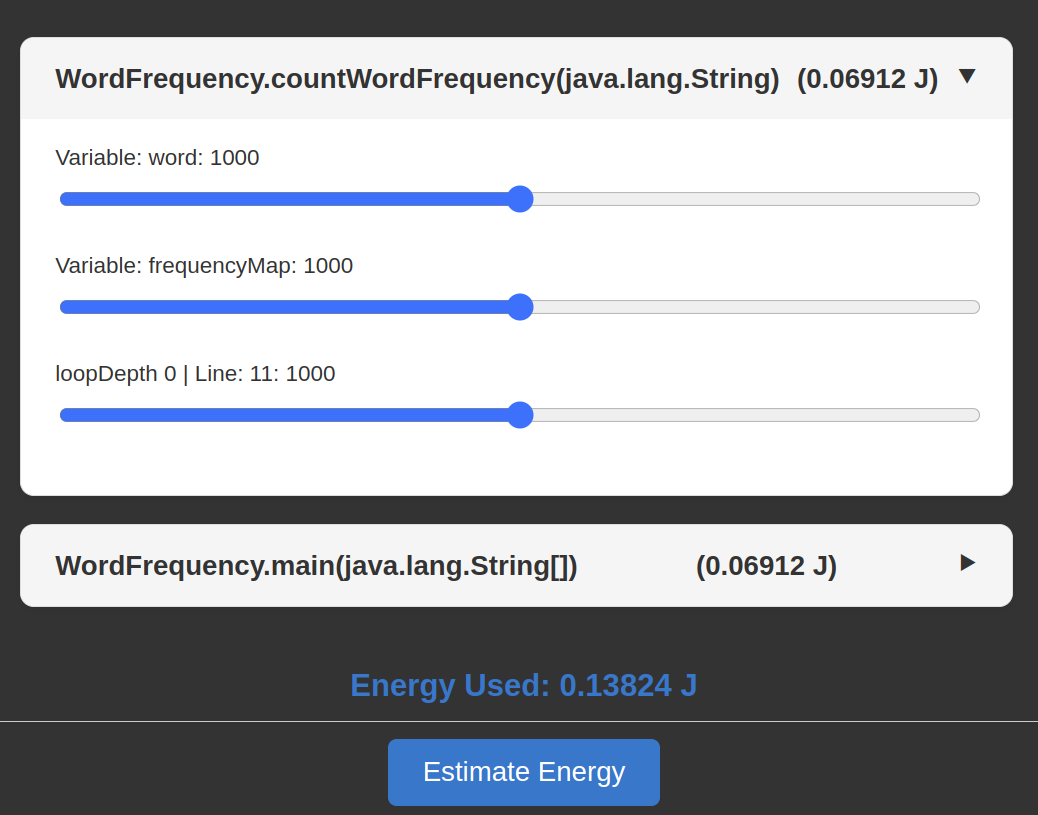
\includegraphics[width = .8 \textwidth]{figures/extension_example2.png}
  \caption{Extension example TreeMap}
  \label{fig:extension_example2}
\end{figure}



\begin{figure}[htbp]
  \centering
  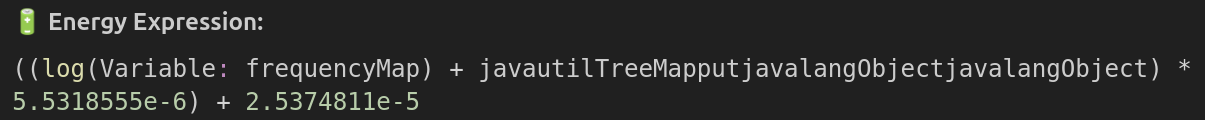
\includegraphics[width = .8 \textwidth]{figures/extension_expression_example.png}
  \caption{Expression for method Map.put(Object, Object)}
  \label{fig:extension_expression_example}
\end{figure}

There is also a feature that can help the user understand how the energy changes. When the mouse hovers through some methods, it is possible to see the mathematical expression utilized for the calculations. The figure ~\ref{fig:extension_expression_example} shows how the expression is displayed in the extension UI. It has the numbers that the model think are the best to predict the energy, and it has the features/variables that it affects the prediction the most. In this case the 2 variables are the size of the map collection and if there are any \texttt{TreeMap} collection being used. This can help understand what are the variables that actually impact the energy of the code. 

The extension can be open in a java project and gather the total energy used by the user made methods, allowing for a better understanding of the code energy impact. Naturally, the extension is limited by the set of pre-trained models it relies on. If a program uses methods that aren't covered by these models, the extension will report an energy usage of zero, which is inaccurate, as those methods still consume energy.